
This section is devoted to review some of the most important works that are highly related to the research presented in this paper.
%
Firstly, the most important MOEAs paradigms are defined.
%
Thereafter, some relevant classifications of crossover operators are discussed.
%
Finally, the popular Simulated Binary Crossover (SBX) operator, which is used extensively in this paper, is explained in detail.

\subsection{Multi-objective Evolutionary Algorithms}

Through the last years has been created a large number of MOEAs that follows different design principles.
%
In order to better classify them, several taxonomies have been proposed \cite{Joel:BOOK_MOEAs}.
%
Attending to the principles of design, MOEAs can be based on Pareto dominance, indicators and/or decomposition \cite{pilat2010evolutionary}.
%
Currently, none of them have reported a clear advantage over the other ones.
%
Particularly, the experimental validation has been carry out by including the Non-Dominated Sorting Genetic Algorithm (NSGA-II) \cite{Joel:NSGAII}, the MOEA based on Decomposition \cite{Joel:MOEAD}, and the $S$-Metric Selection Evolutionary Multi-objective Optimization Algorithm (SMS-EMOA) \cite{Joel:SMSEMOA}.
%
Therefore, they are representative methods of the domination-based, decomposition-based and indicator-based paradigms, respectively.
%
The following subsections briefly describe each one of these paradigms, as well as the selected methods.

\subsubsection{Domination Based MOEAs - NSGA-II}

One of the most recognized paradigms are the domination based algorithms, particularly this family are based on the application of the dominance relation to design different components of the EAs.
%
Since that the dominance relation does not inherently promotes diversity in the objective space, auxiliary techniques such as niching crowding and/or clustering are usually integrated to obtain an acceptable spread and diversity in the objective space.
%
A critic drawback to implement the dominance relation is that it is seriously affected as the number of objectives increases.
%
Due to this the selection pressure is decremented substantially (exponentially)
%
Some strategies have been developed to deal with this issue,
%

A principall drawback of implement the dominance relation is tharelated with the number of objectives, therefore if the number of function objective increase the selection pressure is decremented substantially, based in this, some strategies have been developed to deal with the many-objective problems.

%
Probably, the most popular technique of this group is the NSGA-II.
%
This algorithm \cite{Joel:NSGAII} implements a special parent selection operator.
%
This operator is based on two mechanisms: fast-non-dominated-sort and crowding.
%
The first one tends to provide a convergence to the Pareto front and the second one promotes the preservation of diversity in the objective space.
%
A current version is the NSGA-III which is designed to deal with many-objective problems \cite{Joel:NSGAIII}.%  \cite{horoba2008benefits}.
%

\subsubsection{Decomposition Based MOEAs - MOEA/D}

Decomposition-based MOEAs \cite{Joel:MOEAD} transform a MOP in a set of single-objective optimization problems that are considered simultaneously.
%
This transformation can be achieved through several approaches.
%
The most popular of them is based in a weighted Tchebycheff function, therefore it is necessary provide weight vectors that are well distributed in the $m-1$ simplex that aims well-spread solutions.
%
However, an important drawback of this kind of approaches is that the quality of the approximations is highly related with the Pareto front shape and the weight vectors.
%

MOEA/D \cite{Joel:MOEAD} is a recently designed decomposition-base MOEA.
%
Its main principles include problem decomposition, weighted aggregation of objectives and mating restrictions through the use of neighborhoods.
%
Particularly, the neighborhoods are considered in the variation operators.
%
A very used variant of the MOEA/D is the MOEA/D-DE, which use the DE operators \cite{price2006differential} and the polynomial mutation operator \cite{hamdan2012distribution} in the reproduction phase, also it has two extra measures for maintaining the population diversity \cite{zhang2009performance}.
%
%However, these two extra mechanisms are not enough to deal with long-term executions.


\subsubsection{Indicator Based MOEAs - SMS-EMOA}
\begin{figure}[t]
\centering
\begin{tabular}{cc}
   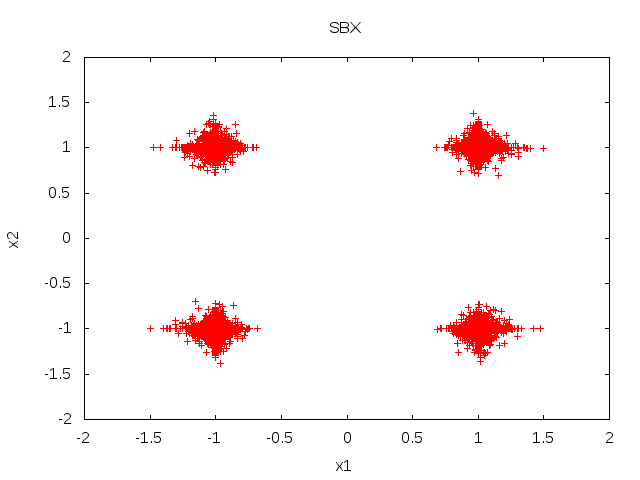
\includegraphics[width=0.25\textwidth]{img/SBX_eta_20_2D.png} 
   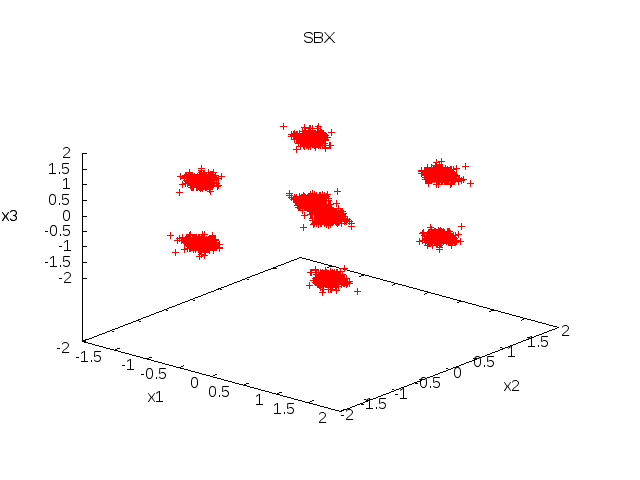
\includegraphics[width=0.25\textwidth]{img/SBX_eta_20_3D.png} 
\end{tabular}
\caption{Simulations of the SBX operator with a distribution index of 20, considering the parents $P_1=(-1.0, -1.0)$ and $P_2=(1.0, 1.0)$ and $P_1=(-1.0, -1.0, -1.0)$ and $P_2=(1.0, 1.0, 1.0)$ for two and three variables respectively.}
\label{fig:Simulations_Index_20}
\end{figure}
In multi-objective optimization several quality indicators have been developed to compare the performance of MOEAs.
%
Since these indicators measure the quality of the approximations attained by MOEAs, a paradigm based on the application of these indicators was proposed.
%
Particularly, instead of dominance concept, the indicators are used in the MOEAs to guide the optimization process.
%
Among the different indicators, hypervolume is a widely accepted Pareto-compliance quality indicator \cite{Joel:IGDPlus_And_GDPlus}.
%
The principal advantage of this algorithms is that the indicator usually takes into account both the quality and diversity of the solutions.
%

A popular and extensively used indicator-based algorithm is the SMS-EMOA \cite{Joel:SMSEMOA}.
%
This algorithm might be considered as hybrid, since it involves an indicator and dominance concepts.
%
Essentially, it integrates the non-dominated sorting method with the use of the hypervolume metric.
%
Thus, SMS-EMOA uses the hypervolume as a density estimator which results in a computationally extensive task.
%
Particularly, the replacement phase erases the individual of the worst ranked front with the minimum contribution to the hypervolume.
%
Taking into account the promising behavior of SMS-EMOA, it has been used in our experimental validation.
%
%
\begin{figure}[!t]
\centering
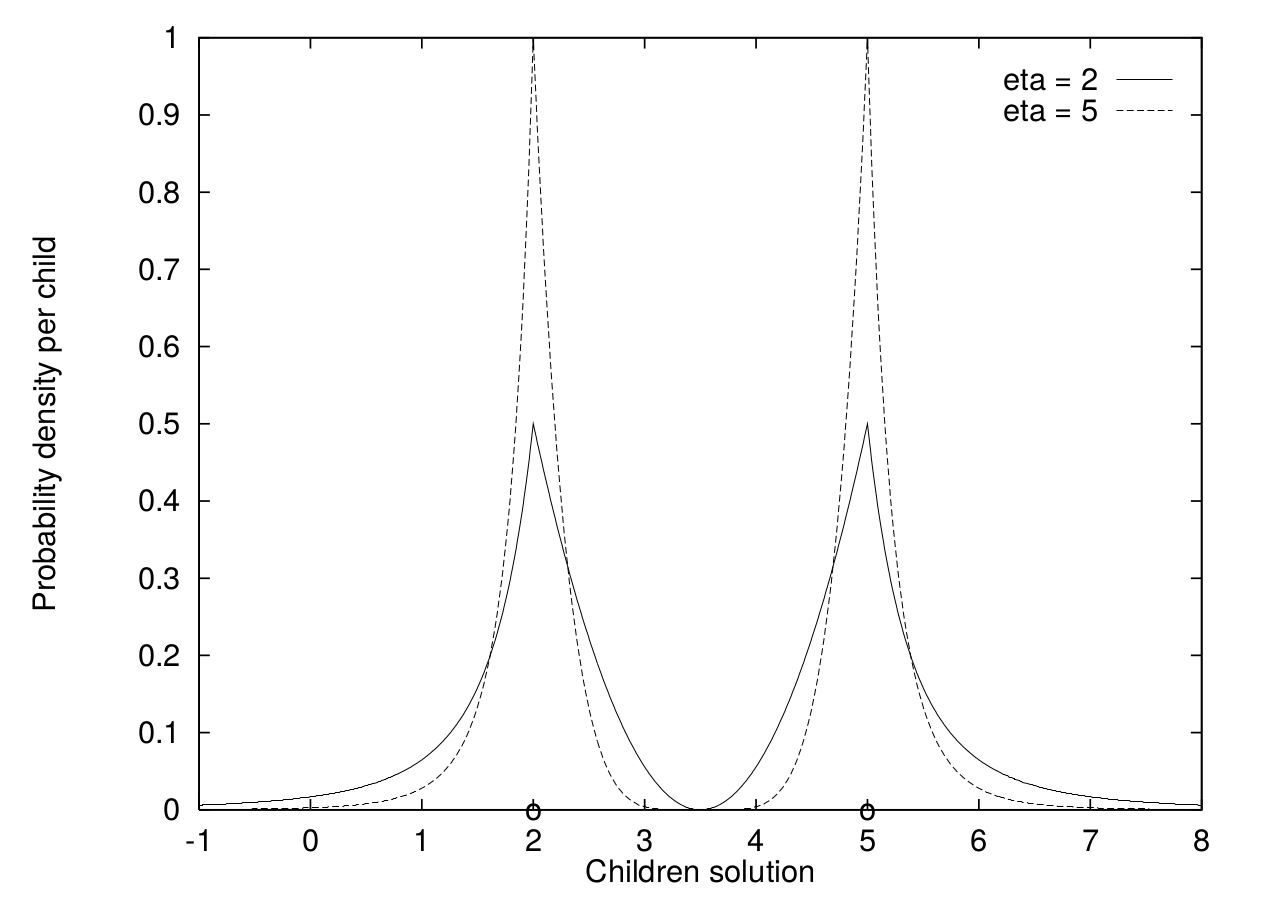
\includegraphics[width=2.5in]{img/DensitySBX_English.png}
\caption{Probability density function of the SBX operator with indexes of distribution 2 and 5. The parents are located in 2 and 5 respectively.}
\label{fig:fig_sim}
\end{figure}
\subsection{Crossover operators}
Crossover operators are designed to generate offspring solutions using information of the parent solutions.
%
They combine the feature of two or more parent solutions to form children solutions.
%
Since several crossover operators have been proposed, some taxonomies have also been provided.
%
The taxonomies are based on features such as the location of new generated solutions or the relation among the variables.
%

A popular taxonomy classifies crossover operators into variable-wise operators and vector-wise operators.
%
In the variable wise category, each variable from parent solutions is recombined independently with a certain pre-specified probability to create new values.
%
These operators are specially suitable to deal with separable problems.
%
Some operators belonging to this category are the Blend Crossover (BLX) \cite{eshelman1993real}, and the SBX \cite{Joel:SBX1994}.
%
On the other hand, the vector-wise recombination operators are designed to take into account the linkage among variables.
%
They usually perform a linear combination of the variable vectors.
%
Some operators belonging to this category are the Unimodal Normally Distributed Crossover (UNDX) \cite{Joel:UNDX}, and the simplex crossover (SPX) \cite{Joel:DE_Storn_SPX}.
%
Additionally, the crossover operators can be classified as Parent-Centric and Mean-Centric \cite{jain2011parent}.
%
In Parent-Centric operators, children solutions are created around one of the parent solutions, whereas in Mean-Centric operators, children solutions are created mostly around the mean of the participating parent solutions.
%
Among the crossover operators, SBX is probably the most frequently used operator, so this research focuses on this crossover.

\subsubsection{The Simulated Binary Crossover - SBX}

The reproduction operators are one of the most relevant components that influence the search process of the GAs.
%
Specifically, the crossover and mutation operators are highly related with the diversity affecting directly the quality of the solutions.
%
%Particularly, in this paper is discussed the crossover operator.

The Simulated Binary Crossover (SBX) \cite{deb1994simulated} is popularly implemented in GAs \cite{Joel:NSGAII,Joel:SMSEMOA} and is classified as Parent-Centric, meaning that two children values ($c_1$ and $c_2$) are created around the parent values ($p_1$ and $p_2$).
%
Also the process of generate the child values is based in a probability distribution.
%
This distribution is defined by a non-dimensional variable, better known as the spread factor $\beta = |c_1 - c_2 | / |p_1 - p_2|$, indicating the ratio of the spread children values related with the parent values.
%

Additionally, this density function uses a distribution index $\eta_c$ (user-defined control parameter) that alters the exploration capability of the operator.
%
Specifically, a small index induces a larger probability of building children values more dissimilar than parents values, whereas with a high index the probabilities of generating children solutions that are similar to the parents increase as is showed in the Figure \ref{fig:fig_sim}.
%

Principally, the SBX has non-zero probability of creating any number in the search space by recombining any two parent values from the search space.
%
The probability distribution to create an offspring value is defined as a function of a non-dimensionalized parameter $\beta \in [0, \infty]$ as follows:
%
\begin{equation}
    P(\beta)= 
\begin{cases}
     0.5(\eta_c + 1)\beta^{\eta_c},& \text{if} \quad \beta \leq 1\\
     0.5(\eta_c + 1) \frac{1}{\beta^{\eta_c + 2}} ,& \text{otherwise}
\end{cases}
\end{equation}
%
Based in the mean-preserving property of children values and parent values, the distribution probability has the following properties:
\begin{itemize}
\item Both offspring values are equi-distant from parent values.
\item There exist a non-zero probability to create offspring solutions in the entire feasible space  from any two parent values.
\item The overall probability of creating a pair offspring values within the range of parent values is identical to the overall probability of creating two offspring values outside  the range of parent values.
\end{itemize}

\begin{figure}[t]
\centering
\begin{tabular}{cc}
   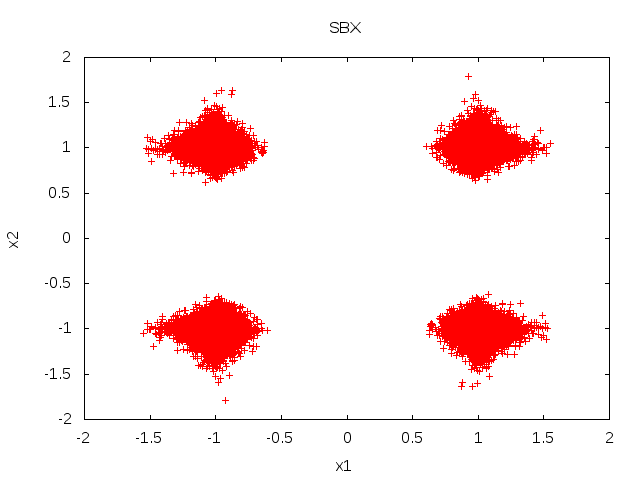
\includegraphics[width=0.25\textwidth]{img/SBX_eta_20_2D_pv_1.png} 
   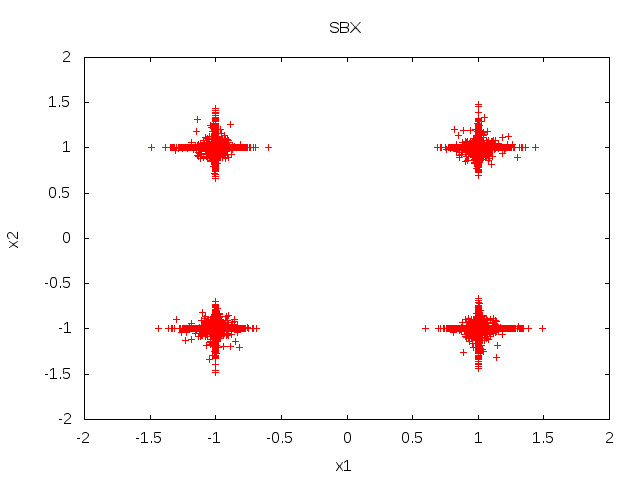
\includegraphics[width=0.25\textwidth]{img/SBX_eta_20_2D_pv_01.png} 
\end{tabular}
\caption{Simulations of the SBX operator with a distribution index of 20, the parents are located in $P_1=(-1.0, -1.0)$ and $P_2=(1.0, 1.0)$. The left simulation corresponds to a probability of altering a variable ($\delta_1$ in Algorithm \ref{alg:SBX_Operator}) to $1.0$ and in the right corresponds to $0.1$.}
\label{fig:Simulation_pv}
\end{figure}





Therefore, considering two participating parent values ($p_1$ and $p_2$), two offspring values ($c_1$ and $c_2$) can be created as linear combination of parent values with a random number $u \in [0, 1]$, as follows:
\begin{equation} 
\begin{split}
c_1 &= 0.5(1 + \beta(u))p_1 + 0.5(1 - \beta(u)) p_2 \\
c_2 &= 0.5(1 - \beta(u))p_1 + 0.5(1 + \beta(u)) p_2
\end{split}
\end{equation}

The parameter $\beta(u)$ depends on the random number $u$, as follows:
\begin{equation}
    \beta(u)= 
\begin{cases}
     (2u)^{\frac{1}{\eta_c+1}},& \text{if} \quad u \leq 0.5,\\
     	(\frac{1}{2(1-u)})^{\frac{1}{\eta_c +1}} ,& \text{otherwise}
\end{cases}
\end{equation}

The above equation only considers a optimization problem having no variable bounds.
%
In most practical problems, each variable is bounded within a lower and upper bound.
%
Thus, Deb and Beyer in 1999 \cite{deb1999self} proposed a modification of the probability distribution showed and is in the Equation (\ref{eq:sbx_spread}).
%
\begin{equation} \label{eq:sbx_spread}
    \beta(u)= 
\begin{cases}
     (2u(1-\gamma))^{\frac{1}{\eta_c+1}},& \text{if} \quad u \leq 0.5/(1-\gamma),\\
     	(\frac{1}{2(1-u(1-\gamma))})^{\frac{1}{\eta_c +1}} ,& \text{otherwise}
\end{cases}
\end{equation}
\begin{equation} \label{eq:child_1}
c_1 = 0.5(1 + \beta(u))p_1 + 0.5(1-\beta(u))p_2
\end{equation}
\begin{equation} \label{eq:child_2}
c_2 = 0.5(1 + \beta(u))p_1 + 0.5(1-\beta(u))p_2
\end{equation}
where the child $c_1$ which is nearest to $p_1$ is calculated according the Equation (\ref{eq:child_1}).
%
Therefore, for $p_1 < p_2$ and the lower bound $a$ is closer to $p_1$ than to $p_2$, thus $\gamma = 1/(\alpha^{\eta_c + 1})$, where $\alpha = 1 + (p_1 - a) / (p_2 - p_1)$.
%
Similarly, the second child $c_2$ is computed with $\alpha = 1 + (b-p_2)/(p_2 - p_1)$, where $b$ correspond to the upper bound.
%
Then, the second child is computed as is indicated in the Equation (\ref{eq:child_2}).
\begin{algorithm}[t]
\algsetup{linenosize=\tiny}
\scriptsize
\caption{Simulated Binary Crossover (SBX)}
\label{alg:SBX_Operator}
\begin{algorithmic}[1]
    \STATE Input: Parents ($P_{1}, P_{2}$), Distribution index ($\eta_c$), Probability distribution ($P_c$).
    \STATE Output: Children ($C_{1}, C_{2}$).
    \IF{ $U[0, 1] \leq P_c$}
       \FOR{ each variable d}
	\IF{ $U[0, 1] \leq  \delta_1$} \label{alg:inherit_variable}
		\STATE Generate $C_{1,d}$ with Equations (\ref{eq:sbx_spread}) and (\ref{eq:child_1}).
		\STATE Generate $C_{2,d}$ with Equations (\ref{eq:sbx_spread}) and (\ref{eq:child_2}).
		 \IF{$ U[0, 1]  \geq  \delta_2 $} 
			\STATE Swap $C_{1,d}$ with $C_{2,d}$.
		 \ENDIF
        \ELSE
	   \STATE $C_{1,d} = P_{1, d}$.
	   \STATE $C_{2,d} = P_{2, d}$.
        \ENDIF
       \ENDFOR
    \ELSE
	\STATE $C_{1,d} = P_{1,d}$.
	\STATE $C_{2,d} = P_{2,d}$.
    \ENDIF
\end{algorithmic}
\end{algorithm}
In the literature \cite{Joel:SBX1994} is not entirely studied the SBX extension to multi-variables problems, in fact the authors implemented a similar mechanism to the uniform crossover for multiple variables \cite{Joel:UNDX} for choosing which variables to cross.
%
However those authors recognized the important implications with the linkage issues, therefore it does not alleviate the linkage problem of some MOPs.
%

\subsubsection{Implementation and analyses of SBX operator}
This section discusses the principal characteristics of SBX operator.
%
Essentially, the behavior of operator is directly affected by three key components.
%
Firstly, it applies a probability of altering each variable which is fixed to $0.5$, therefore in average the half of each parent is copied to each child.
%
Increasing this probability value induces more dissimilar children values, since that in average more variables are modified.
%
An appropriate setting of this probability is related with the MOP, therefore a high probability value is better with objective functions that have high dependence level in the parameters, due that it provides a rotationally invariant behavior \cite{price2006differential}, this can be noticed in the Figure \ref{fig:Simulation_pv}, where a low probability provokes a bias to the axis, therefore it is an ideal approach for separable problems a difference with a high probability (right simulation) where this could be better in non-separable problems.
%
Also this probability value is related with the distribution index, in fact both components have a direct effect in the similarity between parents and children.
%
Otherwise, a low probability value is suitable for objective functions that are separable \cite{ma2016multiobjective}, due that few decision variables are modified by the crossover operation.
%

The second key component consists that two offspring values are interchanged through a probability of $0.5$, in some contexts this probability is known as ``Variable uniform crossover probability'' \cite{tuvsar2007differential} or ``Discrete Recombination'' \cite{muhlenbein1993predictive}.
%
Although that in single-objective this action provides auto-adaptive behavior, in multi-objective optimization could not provide a desirable effect at first stages, the principal reason is that it could be highly disruptive.
%
This components has serial implications, since that interchange variables between the children has the effect of multiple ``reflections'' in the feasible space.
%
However, increasing the dimensions of the decision variables has the effect of increase exponentially the number of reflections ($2^{n}-2$) as is showed in the figure \ref{fig:Simulations_Index_20} where is considered two and three decision variables.
%

Finally, the last component is the distribution index, which plays an important role, since a low index results in a greater exploration level than considering a high distribution index, in fact a distribution index of the unity has a similar effect of the Fuzzy Recombination Operator \cite{voigt1995fuzzy}, the effect of the index can be analyzed in the figure \ref{fig:Simulation_Case_3} where in the left is a simulation with a low index which implies to create more dissimilar children, also can be noticed that it has a bias of create children according to the axis.
%

%
For simplicity the SBX implementation is showed in the Algorithm \ref{alg:SBX_Operator}, which is based in the most frequently used implementation integrated in the NSGA-II code published by Deb et al. \cite{Joel:NSGAII}.
%
It requires two parents ($P_1$ and $P_2$) and create two children ($C_1$ and $C_2$).
%

Principally, the first and second key components correspond to the lines 5 and 8 respectively. 
%
As is usual, the SBX is configured with $\delta_1 = \delta_2 = 0.5$ and $\eta_c = 20$.
%
It is important take into account that this configuration neither considers the dimension of the decision variables space or the criteria stop.

\begin{figure}[t]
\centering
\begin{tabular}{c}
   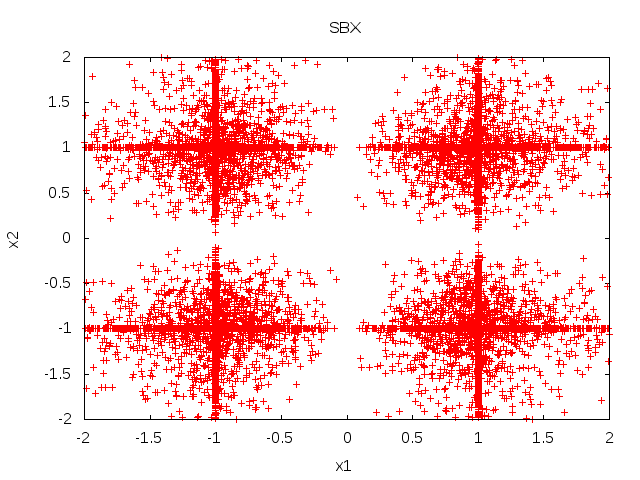
\includegraphics[width=0.24\textwidth]{img/SBX_eta_2.png}  %&
   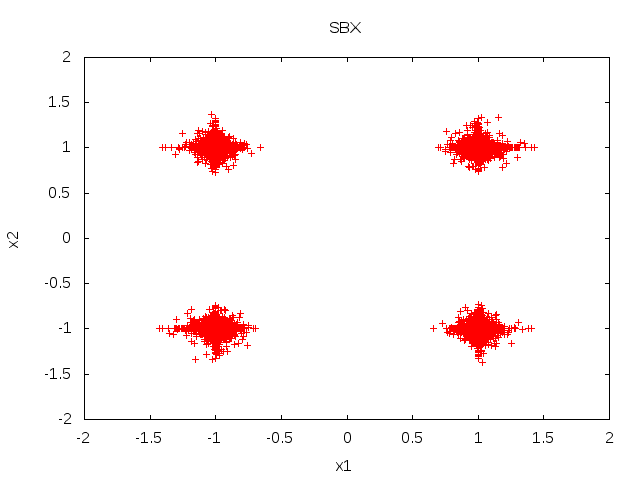
\includegraphics[width=0.24\textwidth]{img/SBX_eta_20.png} 
\end{tabular}
\caption{Simulation the SBX operator with $10,000$ children values, where the parents are located in $P_1=(-1.0, -1.0)$ and $P_2=(1.0, 1.0)$. The left and right are with a distribution index of $2$ and $20$ respectively.}
\label{fig:Simulation_Case_3}
\end{figure}
